\documentclass[12pt, a4paper]{article}

% --- Packages ---
\usepackage[utf8]{inputenc}
\usepackage[margin=1in]{geometry} % Standard margins
\usepackage{graphicx} % To include images/schematics
\usepackage{amsmath} % For mathematical formulas
\usepackage{titlesec} % For custom section styling
\usepackage{booktabs} % For professional-looking tables
\usepackage{fancyhdr} % For headers and footers
\usepackage{tikz}
\usetikzlibrary{shapes,arrows.meta,positioning,calc}
\usepackage{pgfplots}
\usepackage{setspace}
\doublespacing
\usepackage{listings}
\usepackage{xcolor}
\usepackage{float}
\usepackage[hidelinks]{hyperref}

\definecolor{codegreen}{rgb}{0.13,0.55,0.13}
\definecolor{codegray}{rgb}{0.5,0.5,0.5}
\definecolor{codepurple}{rgb}{0.58,0,0.82}
\definecolor{codeblue}{rgb}{0.13,0.29,0.53}
\definecolor{backcolour}{rgb}{0.97,0.97,0.97}
\definecolor{stringcolor}{rgb}{0.63,0.13,0.94}

\lstdefinestyle{matlabstyle}{
    backgroundcolor=\color{backcolour},
    commentstyle=\color{codegreen}\itshape,
    keywordstyle=\color{codeblue}\bfseries,
    numberstyle=\tiny\color{codegray},
    stringstyle=\color{stringcolor},
    basicstyle=\ttfamily\footnotesize,
    breakatwhitespace=false,
    breaklines=true,
    captionpos=b,
    keepspaces=true,
    numbers=left,
    numbersep=8pt,
    showspaces=false,
    showstringspaces=false,
    showtabs=false,
    tabsize=4,
    frame=single,
    framerule=0.5pt,
    rulecolor=\color{codegray},
    xleftmargin=15pt,
    framexleftmargin=15pt,
    language=Matlab
}

\lstset{style=matlabstyle}

% --- Header/Footer Setup ---
\pagestyle{fancy}
\fancyhf{}
\rhead{Spring 2026}
\chead{Signals and Systems Project}
\lhead{\includegraphics[width=1cm]{HU Logo.png}}
\cfoot{\thepage}
\setlength{\headheight}{32.80098pt}
\addtolength{\topmargin}{-20.80098pt}
\pgfplotsset{compat=1.18}
\begin{document}
% --- Title Page ---
\begin{titlepage}
    \centering
    \includegraphics[width=0.6\textwidth]{HU Logo.png}
    \\
    \vspace*{1cm}
    \Large \textbf{EE/CE 252/251 Signals and Systems} \\
    \Large Spring 2026 \\
    \huge \textbf{Milestone 1 Report } \\
    \vfill
    \Large \textbf{Team Members:} \\
    \Large Maaz Haris(mh09633), Rauf Abdullah(ra10307), \& Basil Saeed Bari(bb09892) \\
    \vfill
    \Large \textbf{Instructor:} \\
    \Large Mr.Tariq Mumtaz \\
    \vspace{0.8cm}
\end{titlepage}

\newpage % Start the tables on a new page

% --- TABLE OF CONTENTS ---
\tableofcontents
\newpage

% --- TABLE OF FIGURES ---
\listoffigures
\newpage

%%------Main Content--------%
\section{Introduction}
\subsection{Project Objective}
The primary purpose of this project is to study and solve real-life engineering problems related to Signals and Systems using both real measurements and simulated effects. Acoustic instruments produce sound that consists of a fundamental frequency, known as the keynote, along with a series of overtones. By analyzing tones played by instruments such as the cello and trombone, alongside three additional user-selected instruments, this project investigates the distinct frequency characteristics that define each instrument's unique sound. Furthermore, the project explores signal corruption and data recovery, testing the feasibility of restoring original audio data after it has been distorted by faulty recording system components.
\subsection{Methodology}
To achieve these objectives, MATLAB was utilized as the primary computational tool for signal analysis. The investigation began by importing time-domain audio samples and utilizing spectral analysis to estimate their frequency content. By transitioning the data from the time domain to the frequency domain, the fundamental keynotes and their corresponding overtones could be isolated and examined on both linear and logarithmic scales. This frequency-domain analysis was critical for identifying precise overtone offsets caused by physical constraints like string stiffness. For the signal recovery milestones, mathematical models of the corrupting systems—including downsampling and moving average filters—were analyzed to formulate and code appropriate inverse difference equations aimed at retrieving the original data. Through this systematic methodology, complex problems in signal processing were investigated and resolved.

\section{Tasks}
\subsection{Duration of the Recorded Signals (in seconds)}
\subsubsection{Code}
In this we find the total number of samples in each sample, cello and trombone and multiped it with period of the signal to find the duration of the signal as the duration of a signal is given by the following formulas
\begin{align*}
    t & = \frac{Total\ Samples}{Sampling\ Rate}    \\
    t & = Total\ Samples\ \times\ Sampling\ Period
\end{align*}
\begin{lstlisting}[style=matlabstyle]
    %Calculating the number of samples in cello and trombone
    Nc = length(cello.x)
    Nt = length(trombone.x)

    %Calculating the time of each instrument
    Tc = Nc * cello.dt
    Tt = Nt * trombone.dt
    
    fprintf('Length of Cello recording: %.4f seconds\n', Tc);
    fprintf('Length of Trombone recording: %.4f seconds\n', Tt);
\end{lstlisting}
\subsubsection{Results}
Using the above formula and code we found out that the duration of both cello and trombone sounds was 1.338 seconds long.

\subsection{Keynote and Overtone frequencies of the signals}
The acoustic signature of an instrument is defined by its harmonic series, which consists of a fundamental frequency and subsequent overtones. The fundamental frequency, or keynote ($f_0$),is the lowest frequency in the harmonic series and determines the perceived pitch of the sound. Overtones are the higher frequencies that accompany the keynote. The relationship between their amplitudes and phases produces the unique timbre of the instrument. Ideally, for string and wind instruments, these overtones appear at exact integer multiples of the fundamental frequency, modeled by the equation: 
\begin{align*}
    f_k = kf_o, \quad \quad k = 1,2,\dotsc 
\end{align*}

\subsubsection{Code}
In this part we first calculate the  sampling frequency of the signal ($F_s$) measured in Hertz($Hz$). As we are given the sampling period in the data, which is the time between each recorded data point, the sampling frequency is the inverse of the sampling period $F_s = \frac{1}{T_s}$. Then we created a frequency vector from the 0 Hz to the the Nyquist frequency ($F_s/2$) based on the number of samples. Then we used MATLAB's builtin fft function to convert the time domain signal into a frequency domain signal. This function gives me a vector conatining complex numbers that encode both magnitude and phase information of each frequency present in the signal. As the result of fft signal is based on the length on the input signal, we normalized the results to reflect the true physical amplitudes. As fft gives us a two sided spectrum representing both negative and positive frequencies, and negative frequencies have physical meaning, so the second half of the spectrum is removed, but we make sure that the energy of the signal and amplitudes are unchanged. Then we plot the results of this on two different scales, Linear and Logarithmic.
\begin{lstlisting}
    % --- Cello FFT ---
    % Calculating the Sampling frequency
    Fs_cello = 1 / cello.dt;       
    
    %Creating a frequency vector for x axis 
    f_cello = Fs_cello * (0:(Nc/2)) / Nc;
    
    % Computing FFT(Fast Fourier Transform)
    Y_cello = fft(cello.x);               
    
    %Normalizing the signal and considering magnitude of the signal
    P2_cello = abs(Y_cello / Nc);           
    
    %Converting the two sided signal into a single sided signal and making sure
    %that the energy if the signal is conserved
    P1_cello = P2_cello(1:Nc/2+1);          
    P1_cello(2:end-1) = 2 * P1_cello(2:end-1); 
    
    % --- Trombone FFT ---
    % Calculating the Sampling frequency
    Fs_trombone = 1 / trombone.dt;     
    
    %Creating a frequency vector for x axis 
    f_trombone = Fs_trombone * (0:(Nt/2)) / Nt; 
    
    % Computing FFT(Fast Fourier Transform)
    Y_trombone = fft(trombone.x);    
    
    %Normalizing the signal and considering magnitude of the signal
    P2_trombone = abs(Y_trombone / Nt); 
    
    %Converting the two sided signal into a single sided signal and making sure
    %that the energy if the signal is conserved
    P1_trombone = P2_trombone(1:Nt/2+1); 
    P1_trombone(2:end-1) = 2 * P1_trombone(2:end-1);
    
    % --- Plotting Cello (Linear & Logarithmic) ---
    figure('Name', 'Cello Frequency Spectrum');
    plot(f_cello, P1_cello);
    title('Cello Frequency Spectrum (Linear)');
    xlabel('Frequency (Hz)'); ylabel('Magnitude');
    xlim([0 3000]);% Zoom in to see the peaks clearly
    grid on;
    
    figure;
    semilogy(f_cello, P1_cello);
    title('Cello Frequency Spectrum (Logarithmic)');
    xlabel('Frequency (Hz)'); ylabel('Magnitude (Log)');
    xlim([0 3000]);
    grid on;
    
    
    % --- Plotting Trombone (Linear & Logarithmic) ---
    figure('Name', 'Trombone Frequency Spectrum');
    plot(f_trombone, P1_trombone);
    title('Trombone Frequency Spectrum (Linear)');
    xlabel('Frequency (Hz)'); ylabel('Magnitude');
    xlim([0 3000]);
    grid on;
    
    figure
    semilogy(f_trombone, P1_trombone);
    title('Trombone Frequency Spectrum (Logarithmic)');
    xlabel('Frequency (Hz)'); ylabel('Magnitude (Log)');
    xlim([0 3000]);
    grid on;
    \end{lstlisting}
\newpage
\subsubsection{Results and Plots}
\textbf{Cello}
\begin{figure}[H]
    \centering
    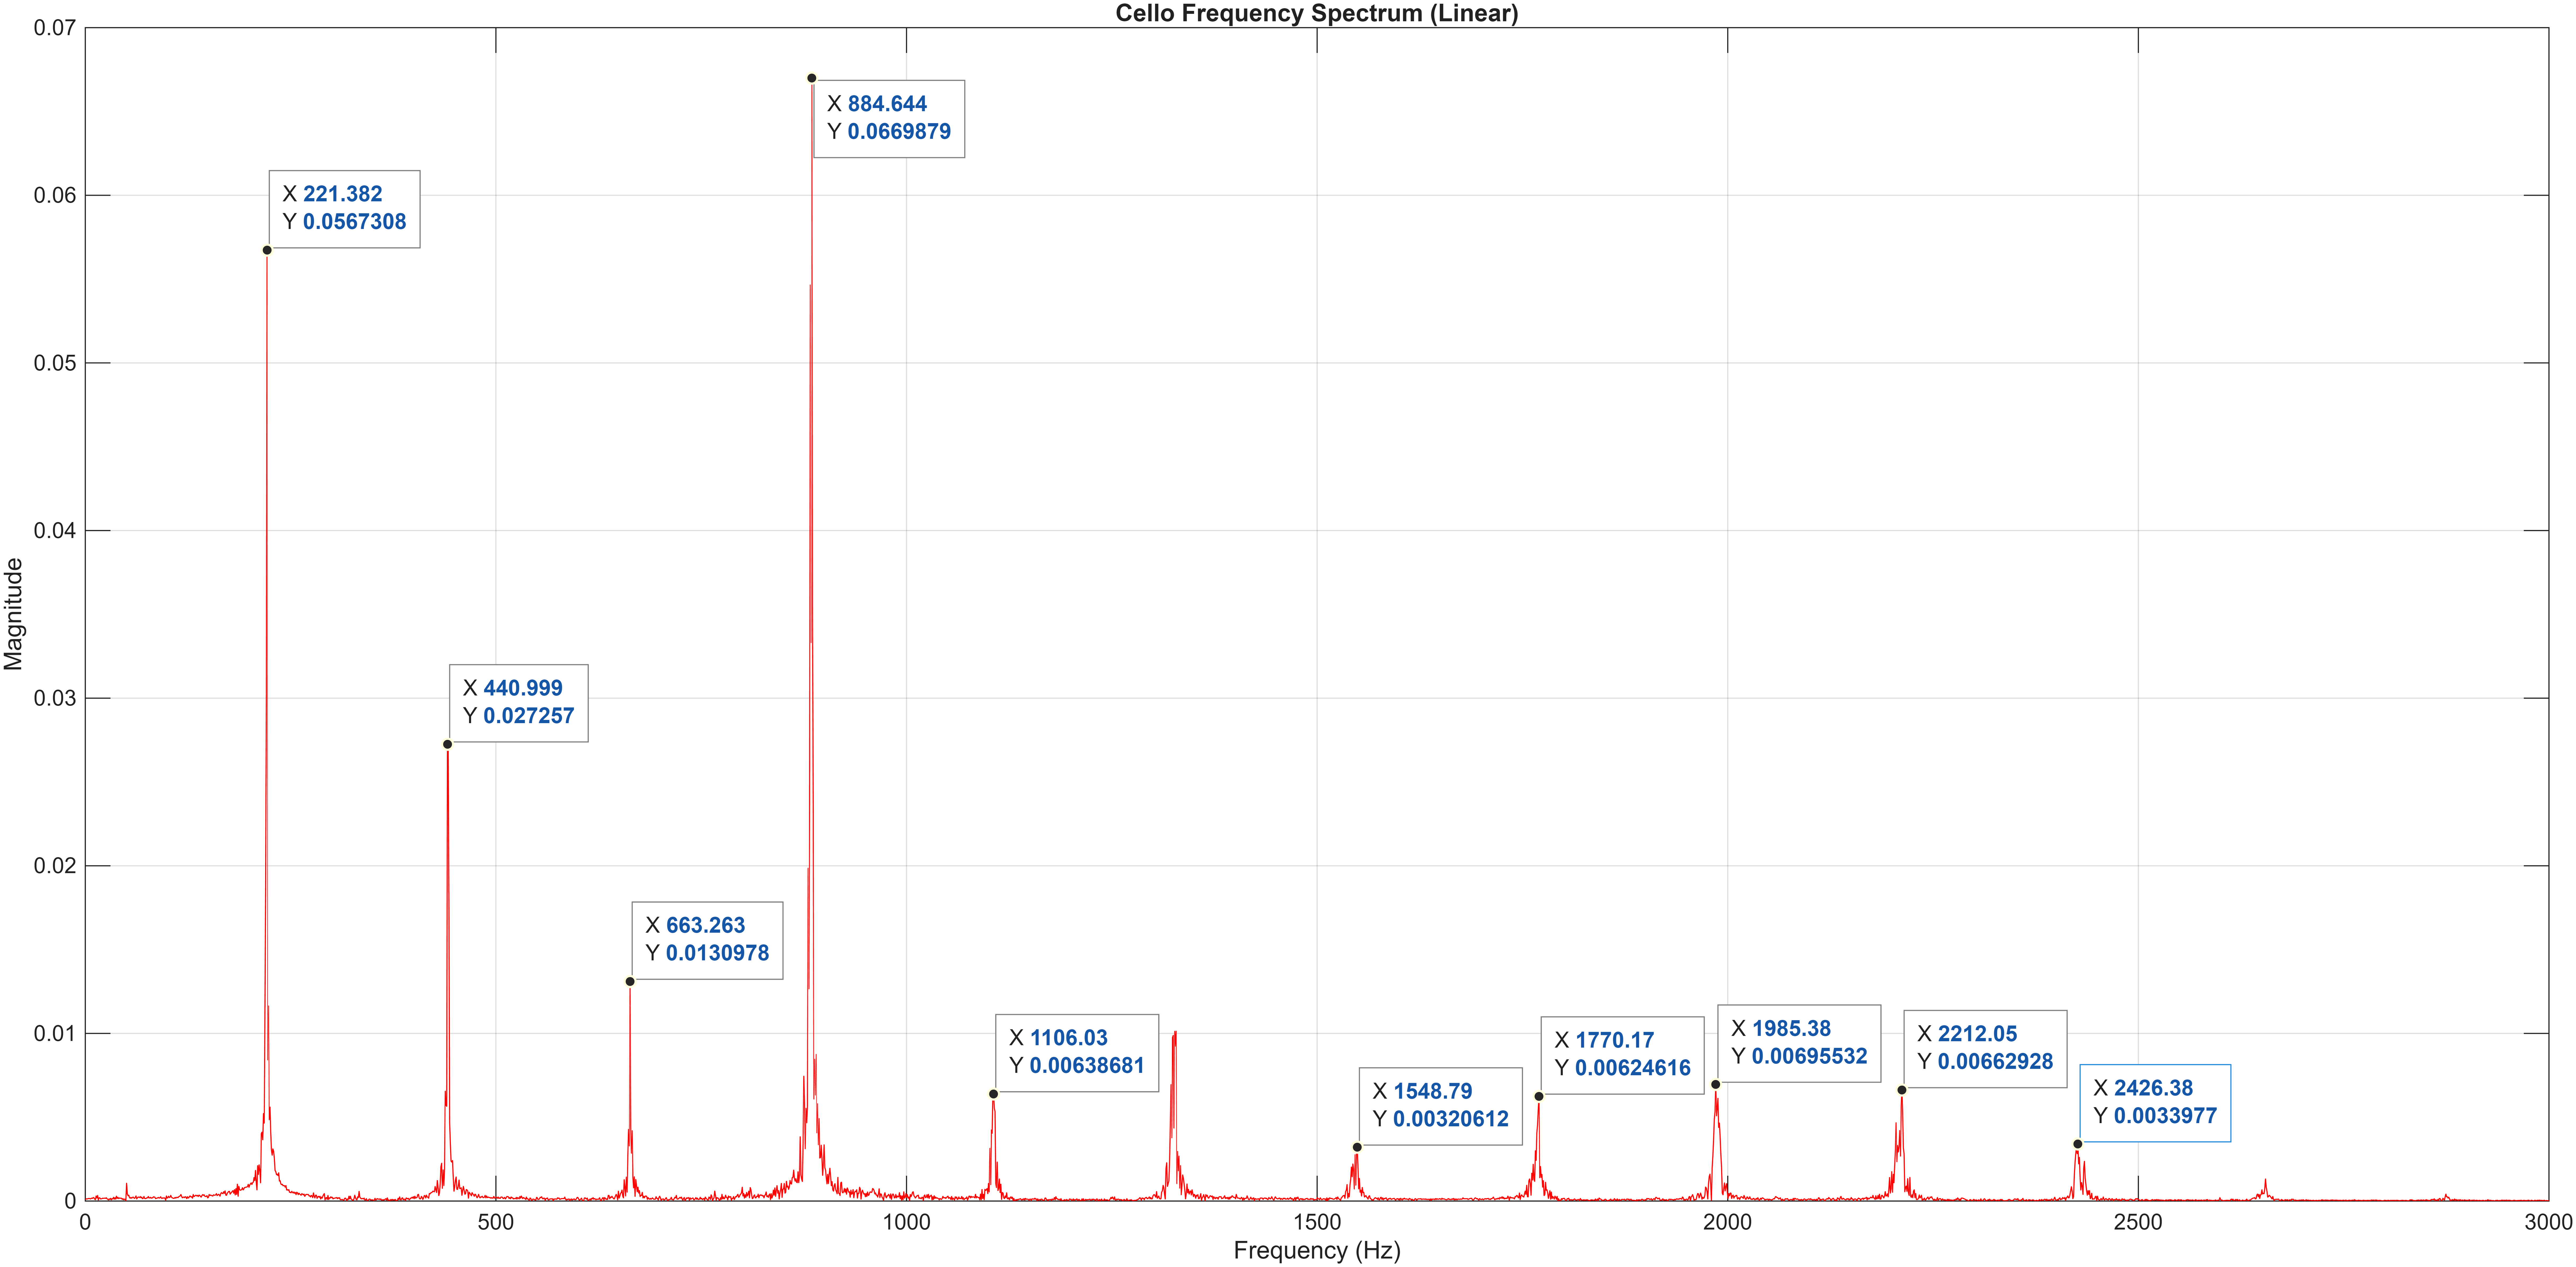
\includegraphics[width=0.95\textwidth]{Cello Frequency Linear.png}
    \caption{Cello Frequencies (Linear)}
    \label{fig:1}
\end{figure}
\begin{figure}[H]
    \centering
    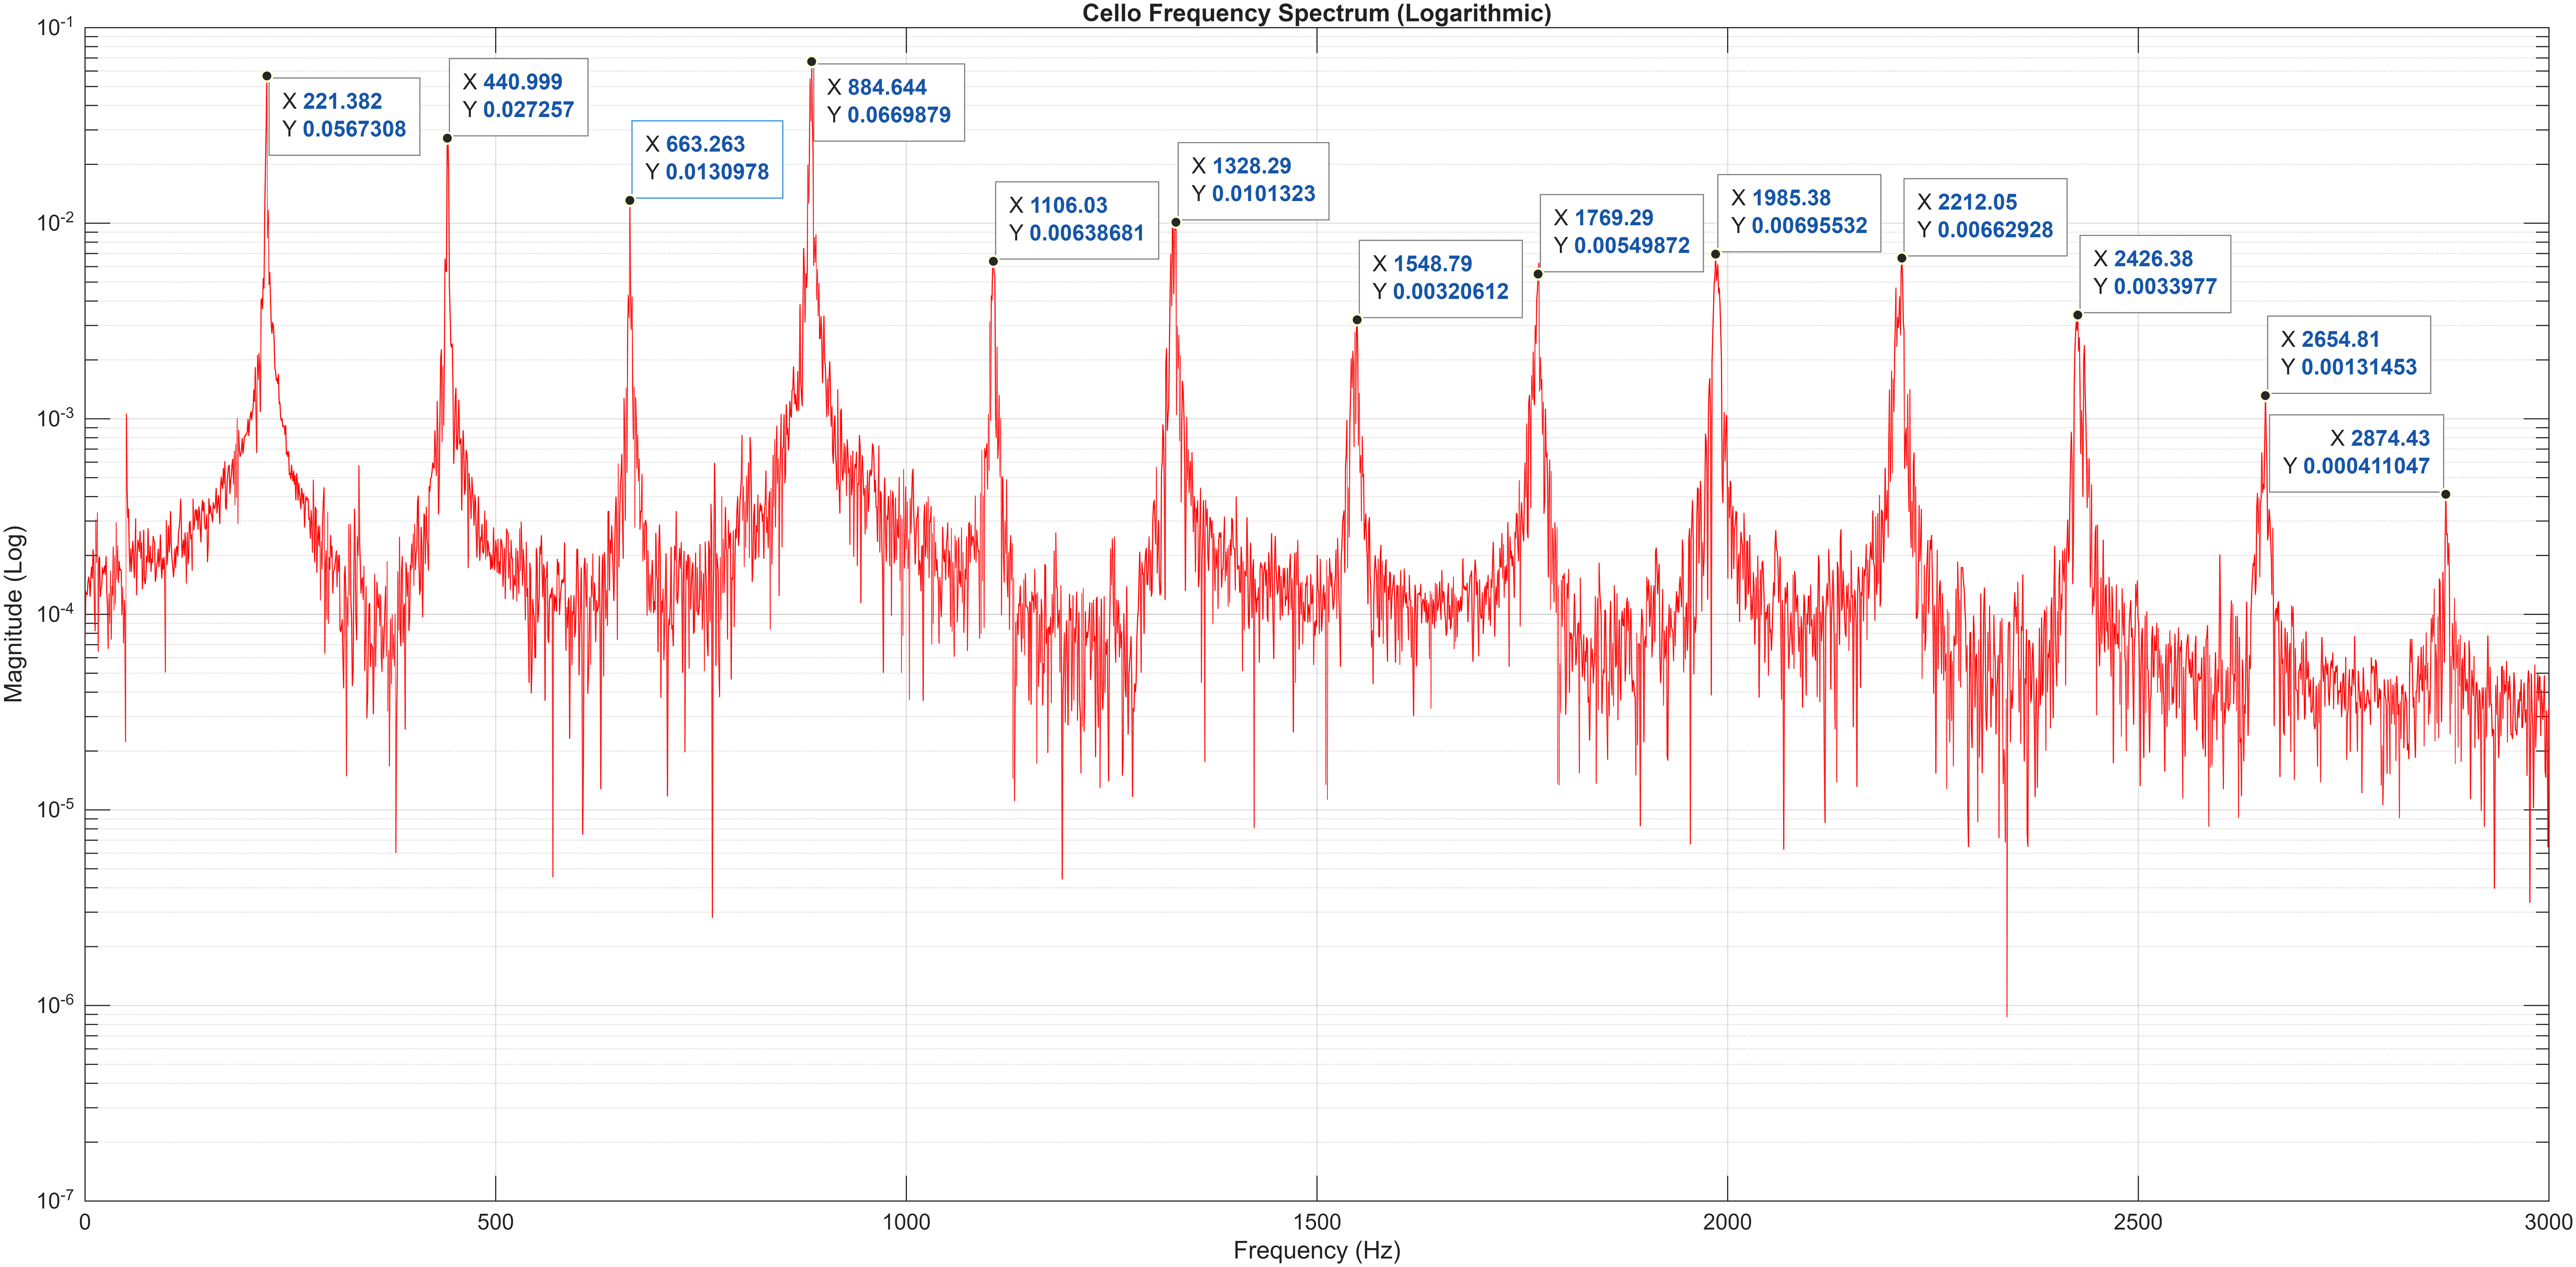
\includegraphics[width=0.95\textwidth]{Cello Frequencies (Logarithm).png}
    \caption{Cello Frequencies (logarithmic)}
    \label{fig:2}
\end{figure}
\begin{itemize}
    \item \textbf{Keynote Frequency:} As observed in the Linear Frequency Spectrum (\autoref{fig:1}), the keynote frequency of Cello is $221.382\ Hz$
    \item \textbf{Overtones: }Using the formula $f_k = kf_0$, we found that the predicted overtone frequencies of the cello signal are $f_1 = 442.764\ Hz,\ f_2 = 664.146\ Hz,\ f_3 = 885.528$.
    However the overtones found using the Linear Frequency Spectrum (\autoref{fig:1}), we found that the overtones are $f_1 = 440.999\ Hz,\ f_2 = 663.262\ Hz,\ f_3 = 884.644\ Hz$. As we can see that the the overtone frequencies observed are not the exact multiple of the  keynote frequency. This offset is due to the stiffness of the string and the model of the overtones taking stiffness into account is 
    \begin{align*}
        f_k = kf_0\sqrt{1 + Bk^2}
    \end{align*}
    (where B is the positive stiffness parameter).
    \item \textbf{Number of Overtones:} As Overtones carry significantly less energy, the Logarithmic Frequency Spectrum is required to accurately count them. Using the logarithmic Spectrum of Cello (\autoref{fig:2}), there are 12 distinct overtones clearly visible above the noise floor. 
\end{itemize}
\textbf{Trombone} 
\begin{figure}[H]
    \centering
    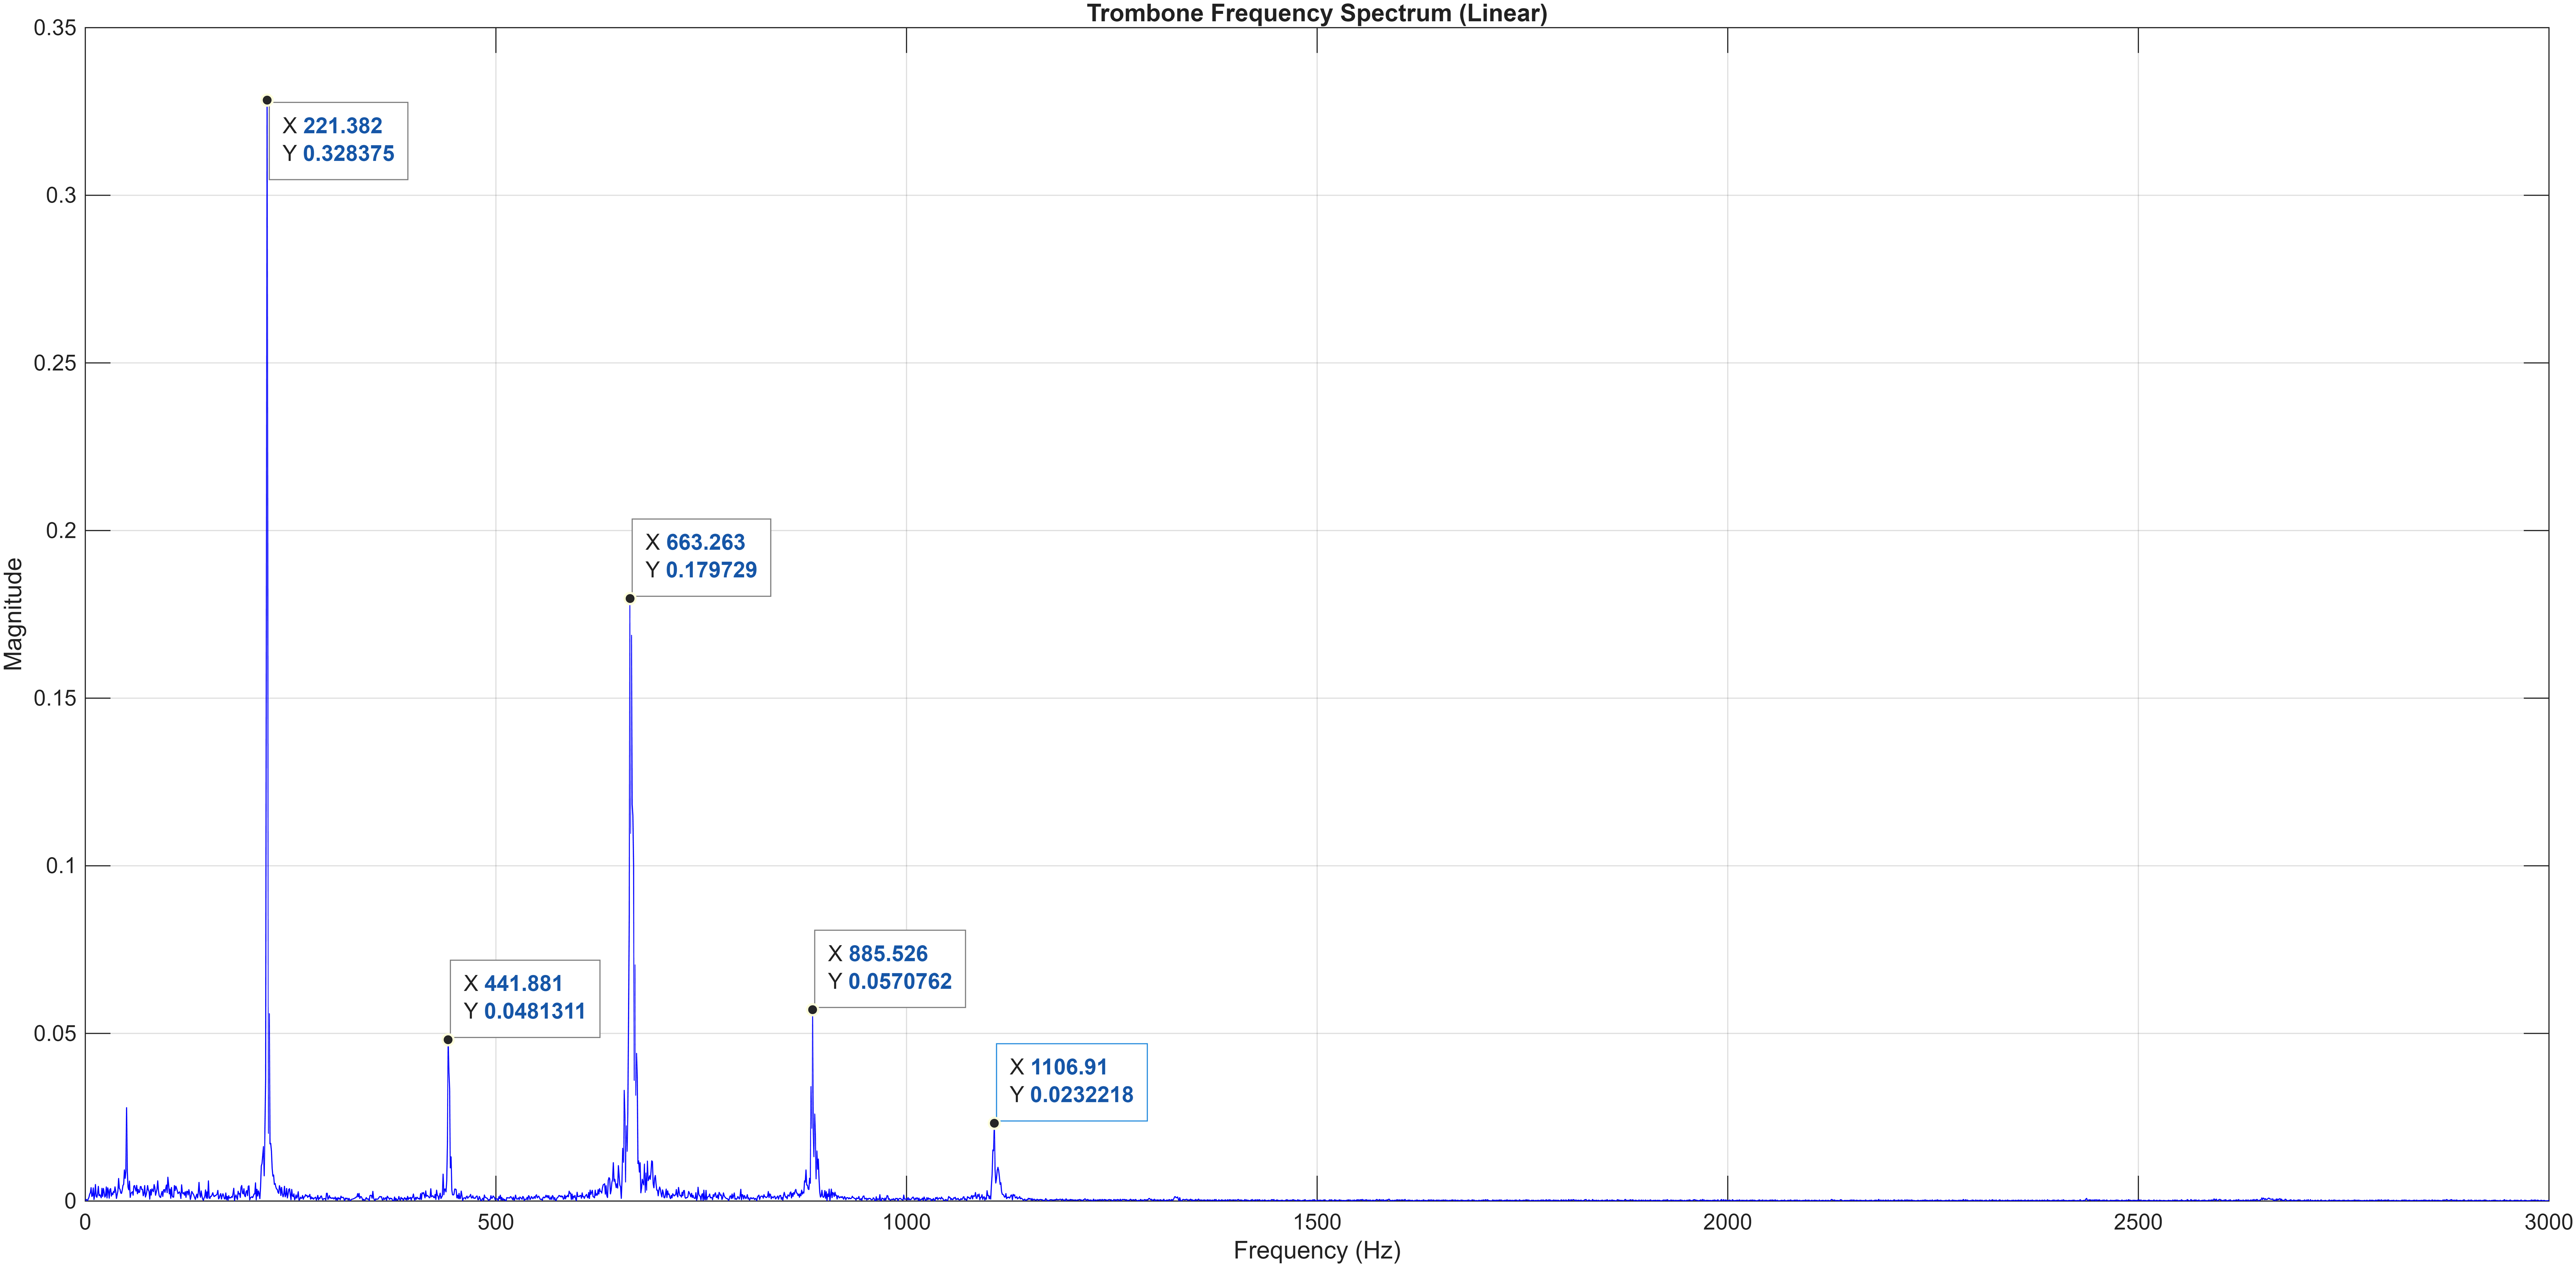
\includegraphics[width=0.95\textwidth]{Trombone Frequency (Linear).png}
    \caption{Trombone Frequency (Linear)}
    \label{fig:3}
\end{figure}
\begin{figure}[H]
    \centering
    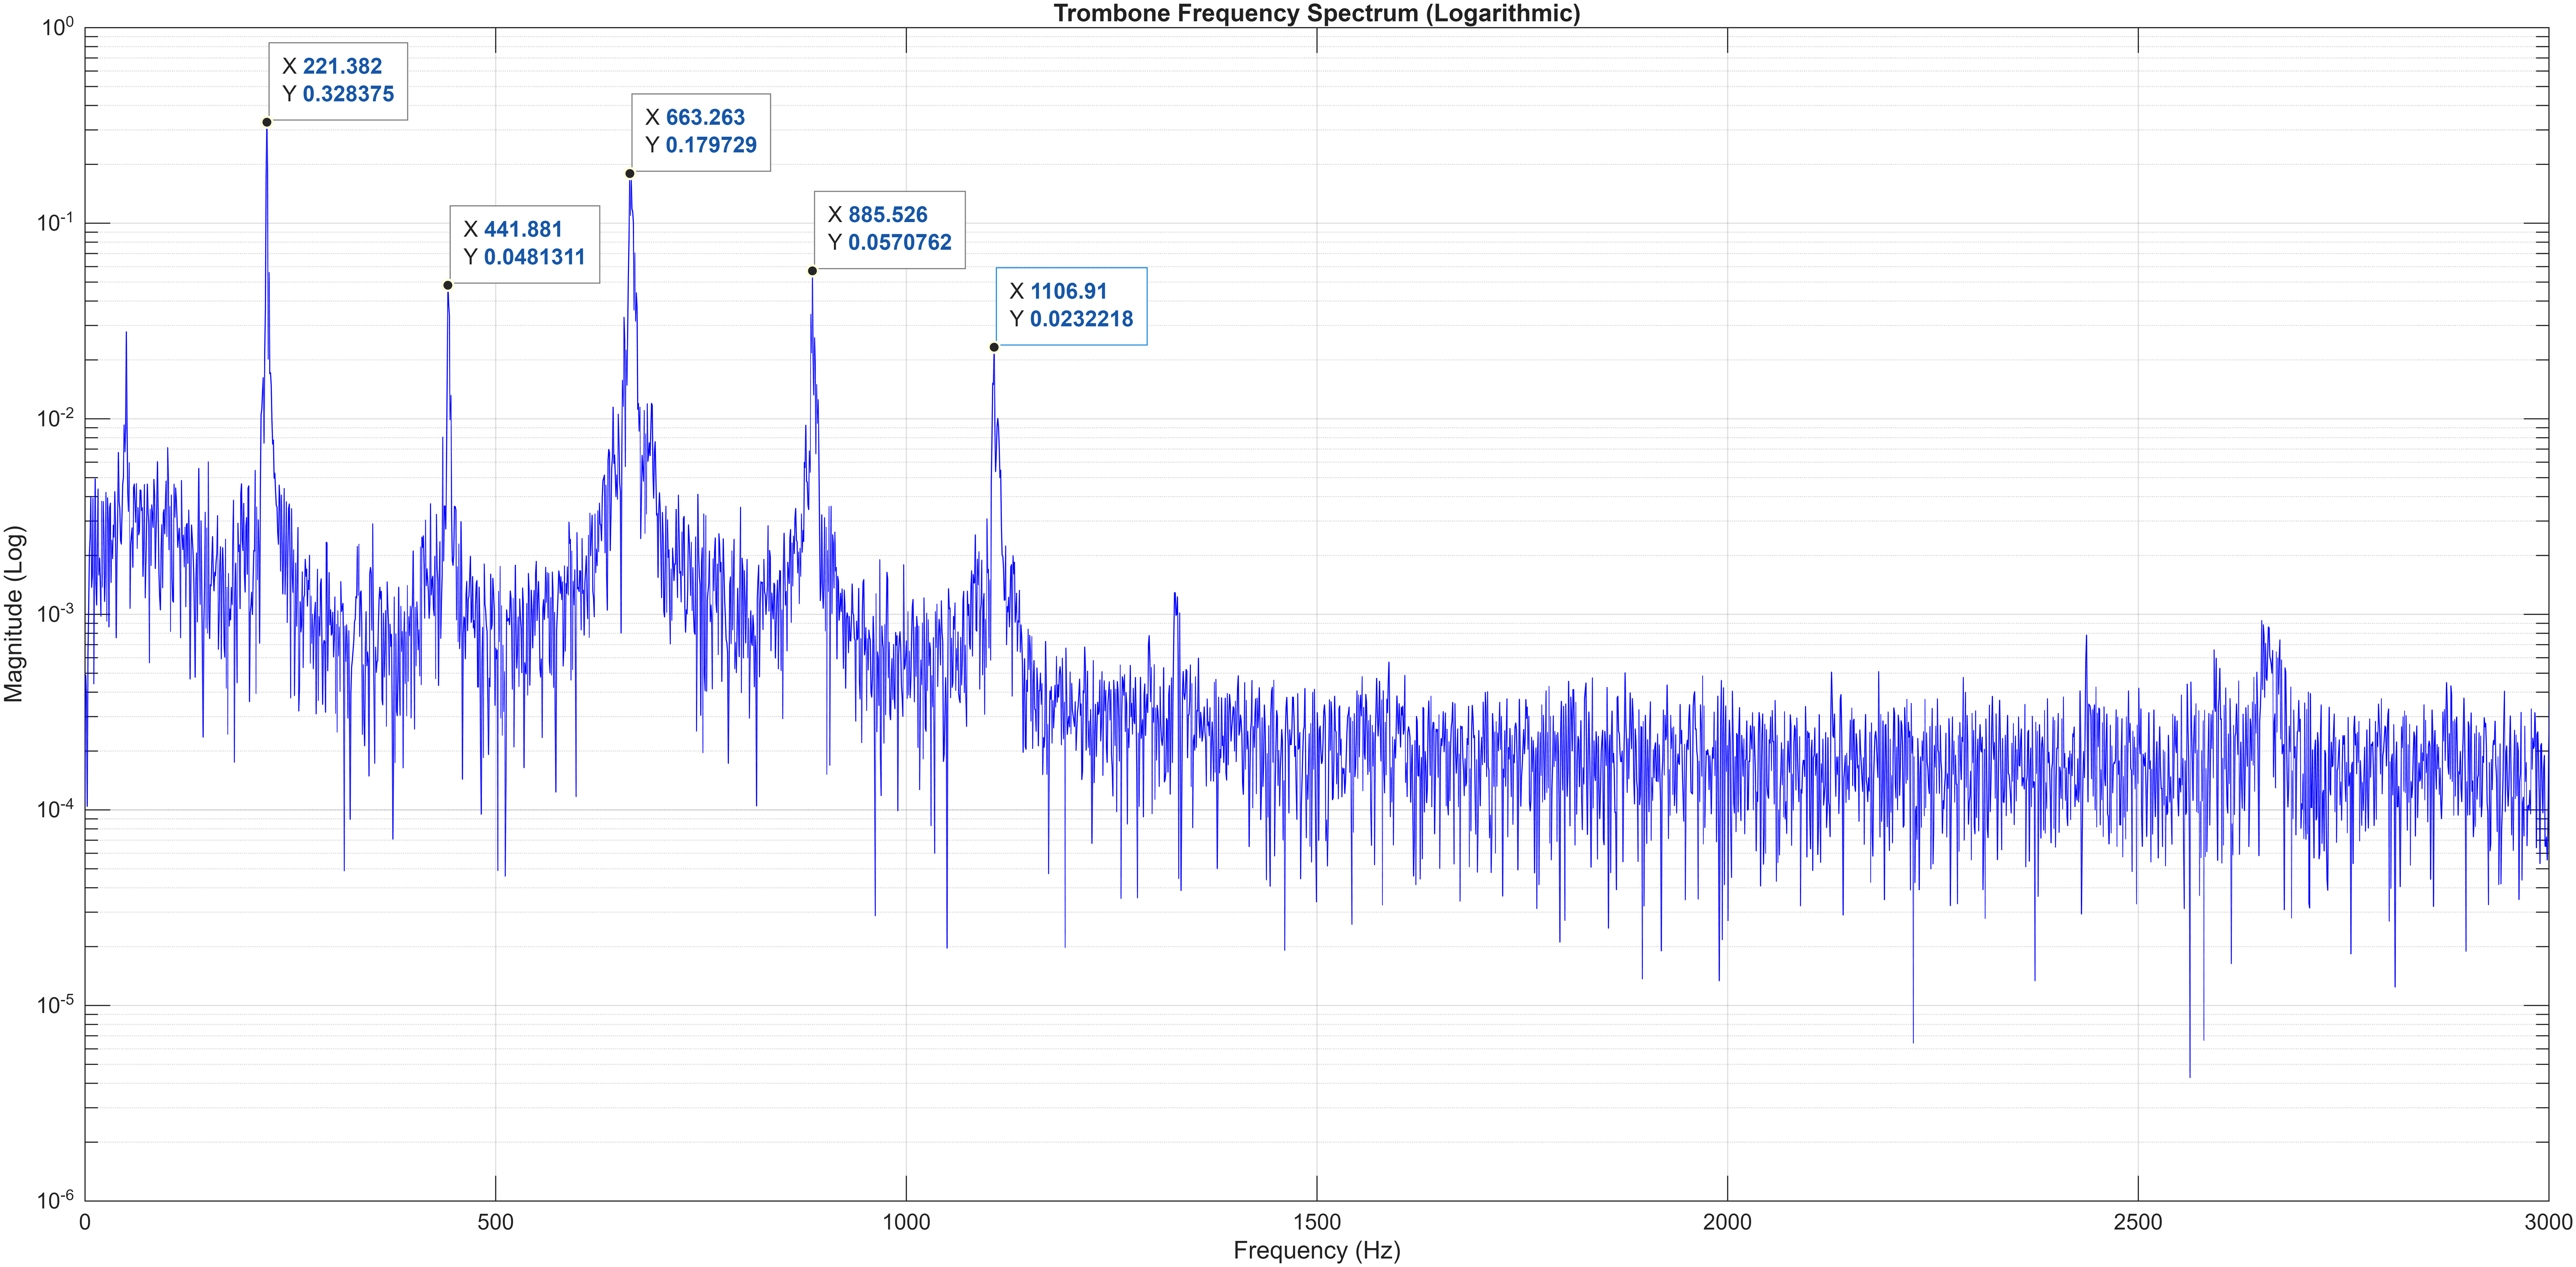
\includegraphics[width=0.95\textwidth]{Trombone Frequency (Logarithmic).png}
    \caption{Trombone Frequencies (logarithmic)}
    \label{fig:4}
\end{figure}
\begin{itemize}
    \item \textbf{Keynote Frequency:} As observed in the Linear Frequency Spectrum (\autoref{fig:3}), the keynote frequency of Cello is $221.382\ Hz$
    \item \textbf{Overtones: }Using the formula $f_k = kf_0$, we found that the predicted overtone frequencies of the cello signal are $f_1 = 442.764\ Hz,\ f_2 = 664.146\ Hz,\ f_3 = 885.528$.
    However the overtones found using the Linear Frequency Spectrum (\autoref{fig:3}), we found that the overtones are $f_1 = 441.881\ Hz,\ f_2 = 663.262\ Hz,\ f_3 = 885.526\ Hz$. As we can see that the the overtone frequencies observed are not the exact multiple of the  keynote frequency. This offset is due to the stiffness of the string and the model of the overtones taking stiffness into account is 
    \begin{align*}
        f_k = kf_0\sqrt{1 + Bk^2}
    \end{align*}
    (where B is the positive stiffness parameter)
    \item \textbf{Number of Overtones:} As Overtones carry significantly less energy, the Logarithmic Frequency Spectrum is required to accurately count them. Using the logarithmic Spectrum of Cello (\autoref{fig:4}), there are 4 distinct overtones clearly visible above the noise floor.
\end{itemize}

\subsection{Signal Corruption and Regeneration}

This section investigates two distinct corrupting systems applied to the cello and trombone signals respectively. For each instrument, the corrupting system is modeled mathematically, an inverse or recovery procedure is derived, and the result is implemented and verified in MATLAB.

\subsubsection{Cello: Corruption and Partial Recovery}

The cello signal $x_c[n]$ is corrupted according to the formula
\begin{align*}
    y_c[n] = n \cdot x_c[2n+1] + 5, \qquad n = 1, 2, \ldots, N_{\max}
\end{align*}
where $N_{\max} = \lfloor(\text{length}(x_c) - 1)/2\rfloor$. This corruption combines three operations: (i) downsampling, since only the odd-indexed samples $x_c[3], x_c[5], x_c[7], \ldots$ are retained and all even-indexed samples are permanently discarded; (ii) time-varying amplitude scaling, where sample $n$ is multiplied by its index $n$; and (iii) a constant DC offset of $+5$ added to every sample.\\
Because the even-indexed samples are irretrievably lost, full recovery of the original signal is impossible. However, the retained odd-indexed samples can be exactly restored by algebraically inverting the scaling and DC offset. Rearranging the corruption formula gives the partial recovery equation:
\begin{align*}
    \hat{x}_c[2n+1] = \frac{y_c[n] - 5}{n}, \qquad n = 1, 2, \ldots, N_{\max}
\end{align*}
The even-indexed positions remain unknown and are set to zero in the reconstructed timeline. To estimate these missing samples, cubic spline interpolation is applied over the known odd-indexed values. Spline interpolation is preferred over linear interpolation for audio signals as it produces a smooth, differentiable curve that better approximates the underlying continuous waveform.

\subsubsection{Code (Cello)}
\begin{lstlisting}[style=matlabstyle]
% ==========================================
% 6. CELLO CORRUPTION & PARTIAL RECOVERY
% ==========================================
% Formula: CelloCorrupted[n] = n * cello[2n + 1] + 5
N_cello_max = floor((length(cello.x) - 1) / 2);
cello_corrupted = zeros(N_cello_max, 1);

% 6a. Simulate corruption
for n = 1:N_cello_max
    cello_corrupted(n) = n * cello.x(2*n + 1) + 5;
end

% 6b & 6c. Cello Partial Recovery
cello_recovered_partial = zeros(N_cello_max, 1);
for n = 1:N_cello_max
    cello_recovered_partial(n) = (cello_corrupted(n) - 5) / n;
end

% --- VISUALIZATION: Reconstructing the timeline ---
% Map the recovered odd samples back to their original timeline positions.
% The lost even samples will remain as 0.
cello_full_timeline = zeros(length(cello.x), 1);
for n = 1:N_cello_max
    cello_full_timeline(2*n + 1) = cello_recovered_partial(n);
end

% Plotting Original vs. Partially Recovered Cello
figure('Name', 'Cello Partial Recovery Verification');
stem(1:100, cello.x(1:100), 'b', 'marker', 'none'); hold on;
stem(1:100, cello_full_timeline(1:100), 'rx', 'marker', 'none', 'LineWidth', 1.5);
legend('Original Signal', 'Recovered Signal (Zeros at lost indices)');
title('Cello Partial Recovery: Demonstration of Lost Samples');
xlabel('Sample Index (n)'); ylabel('Amplitude'); grid on;
hold off;

% ==========================================
% 6d. CELLO RECONSTRUCTION (INTERPOLATION)
% ==========================================
known_indices = (2 * (1:N_cello_max) + 1)';
known_values  = cello_recovered_partial;
query_indices = (3:known_indices(end))';

% Cubic spline interpolation for smooth audio reconstruction
cello_interpolated = interp1(known_indices, known_values, query_indices, 'spline');

% --- VISUALIZATION ---
figure('Name', 'Cello Interpolation Result');
stem(query_indices(1:150), cello.x(query_indices(1:150)), 'b', ...
     'marker', 'none', 'LineWidth', 1.5); hold on;
stem(query_indices(1:150), cello_interpolated(1:150), 'g', ...
     'marker', 'none', 'LineWidth', 1.5);
legend('Original Cello', 'Interpolated Guess');
title('Cello Recovery via Spline Interpolation (First 150 samples)');
xlabel('Sample Index'); ylabel('Amplitude'); grid on;
hold off;
\end{lstlisting}

\subsubsection{Results and Plots (Cello)}

\begin{figure}[H]
    \centering
    \includegraphics[width=0.95\textwidth]{Cello Partial Recovery.png}
    \caption{Cello Partial Recovery: Demonstration of Lost Samples}
    \label{fig:5}
\end{figure}

\begin{figure}[H]
    \centering
    \includegraphics[width=0.95\textwidth]{Cello Interpolation.png}
    \caption{Cello Recovery via Spline Interpolation (First 150 Samples)}
    \label{fig:6}
\end{figure}

\begin{itemize}
    \item \textbf{Partial Recovery:} As shown in \autoref{fig:5}, at every odd-indexed position the recovered amplitude exactly matches the original signal, confirming that the derived inverse equation correctly inverts the scaling and DC offset. At every even-indexed position the value is zero, demonstrating the permanent information loss caused by the downsampling step of the corruption.

    \item \textbf{Spline Interpolation:} As shown in \autoref{fig:6}, the cubic spline interpolation attempts to estimate the missing even-indexed samples from the surrounding known odd-indexed values. The interpolated signal broadly follows the envelope of the original; however, visible discrepancy may be visible at many positions. This is expected, since interpolation can only estimate information that was permanently discarded by the corruption. The accuracy of the estimate is limited by how rapidly the signal varies between adjacent known samples.
\end{itemize}

\subsubsection{Trombone: Corruption and Full Recovery}

The trombone corrupting system is a causal 2-point moving-average filter:
\begin{align*}
    y_t[n] = \frac{1}{2}\bigl(x_t[n] + x_t[n-1]\bigr), \qquad n \geq 2
\end{align*}
with the initial condition $y_t[1] = \frac{1}{2}\,x_t[1]$, implying $x_t[0] = 0$. Unlike the cello case, no samples are discarded: every sample of $x_t[n]$ contributes to the output $y_t[n]$, so the original signal can be recovered. Rearranging for $x_t[n]$ yields the inverse difference equation:
\begin{align*}
    x_t[n] = 2\,y_t[n] - x_t[n-1], \qquad n \geq 2
\end{align*}
with initial condition $x_t[1] = 2\,y_t[1]$. Here, each recovered sample depends on the current corrupted sample and the previously recovered sample.

\subsubsection{Code (Trombone)}
\begin{lstlisting}[style=matlabstyle]
% ==========================================
% 7. TROMBONE CORRUPTION & FULL RECOVERY
% ==========================================
% Formula: TromboneCorrupted[n] = 0.5*(trombone[n] + trombone[n-1])
trombone_corrupted = zeros(length(trombone.x), 1);

% 7a. Simulate corruption
trombone_corrupted(1) = 0.5 * trombone.x(1);
for n = 2:length(trombone.x)
    trombone_corrupted(n) = 0.5 * (trombone.x(n) + trombone.x(n-1));
end

% 7b & 7c. Trombone Full Recovery
% Inverse difference equation: x[n] = 2*y[n] - x[n-1]
trombone_recovered = zeros(length(trombone_corrupted), 1);
trombone_recovered(1) = 2 * trombone_corrupted(1);
for n = 2:length(trombone_corrupted)
    trombone_recovered(n) = 2 * trombone_corrupted(n) - trombone_recovered(n-1);
end

% Verify recovery success
figure('Name', 'Trombone Recovery Verification');
plot(1:100, trombone.x(1:100), 'b', 'LineWidth', 2); hold on;
plot(1:100, trombone_recovered(1:100), 'r--', 'LineWidth', 1.5);
legend('Original', 'Recovered');
title('Verification of Complete Trombone Recovery');
xlabel('Sample Index (n)'); ylabel('Amplitude'); grid on;
hold off;
\end{lstlisting}

\subsubsection{Results and Plots (Trombone)}

\begin{figure}[H]
    \centering
    \includegraphics[width=0.95\textwidth]{Trombone Recovery.png}
    \caption{Verification of Complete Trombone Recovery}
    \label{fig:7}
\end{figure}

\begin{itemize}
    \item \textbf{Full Recovery:} As observed in \autoref{fig:7}, the recovered trombone signal (red dashed) is completely indistinguishable from the original (blue solid) across all 100 plotted samples. This confirms that the inverse difference equation $x_t[n] = 2\,y_t[n] - x_t[n-1]$ achieves exact recovery, as expected from the fact that no information was lost during the moving-average corruption.

    \item \textbf{Comparison with Cello:} The trombone corruption is a Linear Time-Invariant (LTI) system that preserves all sample information, making exact inversion possible. In contrast, the cello corruption involves an irreversible downsampling step, limiting recovery to a partial reconstruction. 
\end{itemize}
\end{document}
